\documentclass[SE,authoryear,toc,lsstdraft]{lsstdoc}
\input{meta}

% Package imports go here.

% Local commands go here.

%If you want glossaries
%\input{aglossary.tex}
%\makeglossaries

\title{Information Sharing during Commissioning}

% Optional subtitle
% \setDocSubtitle{A subtitle}

\author{
Keith Bechtol, Steve Ritz, and others
}

\setDocRef{SITCOMTN-076}
\setDocUpstreamLocation{\url{https://github.com/lsst-sitcom/sitcomtn-076}}

\date{\vcsDate}

% Optional: name of the document's curator
% \setDocCurator{The Curator of this Document}

\setDocAbstract{%
This document describes what information from the Rubin Observatory Construction Project will be available to the community during the period from LSSTCam integration on the telescope through the start of LSST and release of commissioning data via the Early Science Program.
%This document supplements the
We provide additional details supplementing the Vera C. Rubin Observatory Data Policy and Project Publication Policy to describe appropriate information sharing practices for Rubin Observatory staff and affiliates during the on-sky commissioning period.
This document also includes a proposed set of guidelines for the Rubin Observatory Project Team that are intended to promote the generation and dissemination of high-quality documentation to support the LSST science community.
%, and Rubin Observatory Data Security Standards Implementation
}

% Change history defined here.
% Order: oldest first.
% Fields: VERSION, DATE, DESCRIPTION, OWNER NAME.
% See LPM-51 for version number policy.
\setDocChangeRecord{%
  \addtohist{1}{YYYY-MM-DD}{Unreleased.}{Keith Bechtol}
}


\begin{document}

% Create the title page.
\maketitle
% Frequently for a technote we do not want a title page  uncomment this to remove the title page and changelog.
% use \mkshorttitle to remove the extra pages

% ADD CONTENT HERE
% You can also use the \input command to include several content files.

\begin{warning}[Drafting in progress!]
  This policy document is not yet released.
\end{warning}

\section{Motivation and Scope}

The final stages of the Rubin Observatory Construction Project involving on-sky commissioning and science validation of the integrated system will be an exciting and dynamic time.
During this period, new capabilities will be continuously added and tested.
Our understanding of the technical and scientific performance of the Observatory will be rapidly advancing.
In parallel, the operations team will be preparing to start the LSST 10-year survey and to release on-sky data products to the science community as part of the Early Science Program \citedsp{RTN-011}.

For multiple reasons, Rubin Observatory needs clear and well-publicized policies on information sharing as a function of time during the on-sky commissioning phase.

\begin{enumerate}

  \item The Rubin Observatory has a set of standards for data security.
  The relevant aspects are as follows:
  %The US funding agencies, National Science Foundation (NSF) and Department of Energy (DOE), have provided a set of standards for data security (DMTN-199).

  \begin{itemize}

    \item Delayed public release of focal plane scientific data:
    During commissioning, engineering and imaging data will be embargoed for all non-Project team members for a period of at least 30 days following the observation.
    After this 30 day embargo, only with explicit approval may proprietary information, including data products from commissioning, be shared outside the Project team.
    Data aside from focal plane scientific data may be made available following the Project plan which includes astronomical metadata (within 24 hours), alert postage stamp images (within 60 sec), and weather and sky monitoring data.
    %not corresponding to artificial Earth-orbiting satellites
    %Delay public release of focal plane scientific data for an embargo period of at least 80 hours following the observation.
    %Hold engineering and commissioning imaging data for an embargo period of at least 30 days.

    \item Project team members are required to use only approved Project tools, platforms, and processes for communication, data access and analysis, documentation, software development, work management, etc.
    In practice, we expect most work done by the Project team on the commissioning data to be done within protected directories at the Rubin US Data Facility at SLAC.
    %Embargoed data will remain on designated project computers prior to release.

  \end{itemize}

  \item To maximize opportunities for public engagement, Rubin Observatory will embargo all images prior to major event releases (e.g., the System First Light celebration) as leaks severely compromise public relations effectiveness.

  \item The Rubin Science Community needs timely information about the technical and scientific performance of the as-built system to prepare for their science analyses.

  \item The Project team must be fully enabled to focus on time-sensitive work assignments needed to demonstrate Construction Completeness and Operational Readiness:

  \begin{itemize}

    \item There must exist internal communication channels to maintain free flow of information within the Project team.

    \item The commissioning group will be busy with commissioning tasks and will not be able to answer broader community questions.

  \end{itemize}

\end{enumerate}

This document provides additional details supplementing the Vera C. Rubin Observatory Data Policy \citedsp{RDO-013}, Project Publication Policy \citedsp{LPM-162} to describe appropriate information sharing practices for Rubin Observatory staff and affiliates during the on-sky commissioning period.
% , and Rubin Observatory Data Security Standards Implementation (DMTN-199)

This document also includes a proposed set of guidelines for the Rubin Observatory Project team that are intended to promote the generation and dissemination of high-quality documentation to support the LSST science community.

Definitions:

\begin{itemize}

  \item The \textbf{Project team} includes all individuals working for Rubin Observatory who have access to proprietary engineering and on-sky commissioning data from LSSTCam prior to their release, which includes all Rubin Observatory staff as well as participants in the SIT-Com In-Kind Contribution Programs \citedsp{SITCOMTN-050}.

  \item \textbf{Focal plane scientific data} corresponds to proprietary data products from on-sky imaging with LSSTCam as defined in the Rubin Data Policy \citedsp{RDO-013}.

  \item A \textbf{derived data product} is defined in the Rubin Data Policy \citedsp{RDO-013} as a data product that is derived from LSST proprietary data but that cannot be used to recreate any proprietary LSST data product(s).
  %A representation of an image that cannot be used to recreate the array of pixel values of a proprietary data product (or other equivalent) is considered a derived data product.

  %\item \textbf{Postage stamps} are image cutouts that are $30 \times 30$ arcseconds, centered on an Object, and included in every Alert.

\end{itemize}

The remainder of this document is organized as follows:

\begin{itemize}

  \item Section \ref{early_science} provides an overview of the Early Science Program to place planned data delivery milestones in the context of system integration, commissioning, and verification and validation activities.

  \item Section \ref{policy} describes policy on what information from the Rubin Observatory Construction Project will be available to the community during the period from LSST Camera integration on the telescope through the start of the LSST and release of commissioning data via the Early Science Program.
  We define a process to approve the sharing of derived data products based on commissioning data prior to the associated release using technotes.

  \item Section \ref{publications} discuss publications based on commissioning data, supplementing Vera C. Rubin Observatory Data Policy \citedsp{RDO-013} and Project Publication Policy \citep{LPM-162} with additional details pertinent to the commissioning period.
  We propose guidelines for the Project team to promote the generation and dissemination of high-quality documentation on the scientific performance.

  \item Section \ref{operations} concludes with brief comments regarding the transition to Operations.

\end{itemize}

\section{Early Science Program}
\label{early_science}

Rubin Observatory has planned an Early Science Program to enable high-impact science prior to the first annual data release of the LSST \citedsp{RTN-011}.
Components of the Early Science Program include releasing science-grade commissioning data products via a series of Data Previews, ramping up of the transient alert stream during commissioning, implementing a program of incremental template generation to augment alert production in the early phases of the survey, and the first LSST Data Release, DR1, based on the first 6 months of data from the LSST.

Figure \ref{timeline} shows an overview of the expected timeline for release of Early Science data products and supporting documentation for the technical and scientific performance of Rubin Observatory.

\begin{figure}
  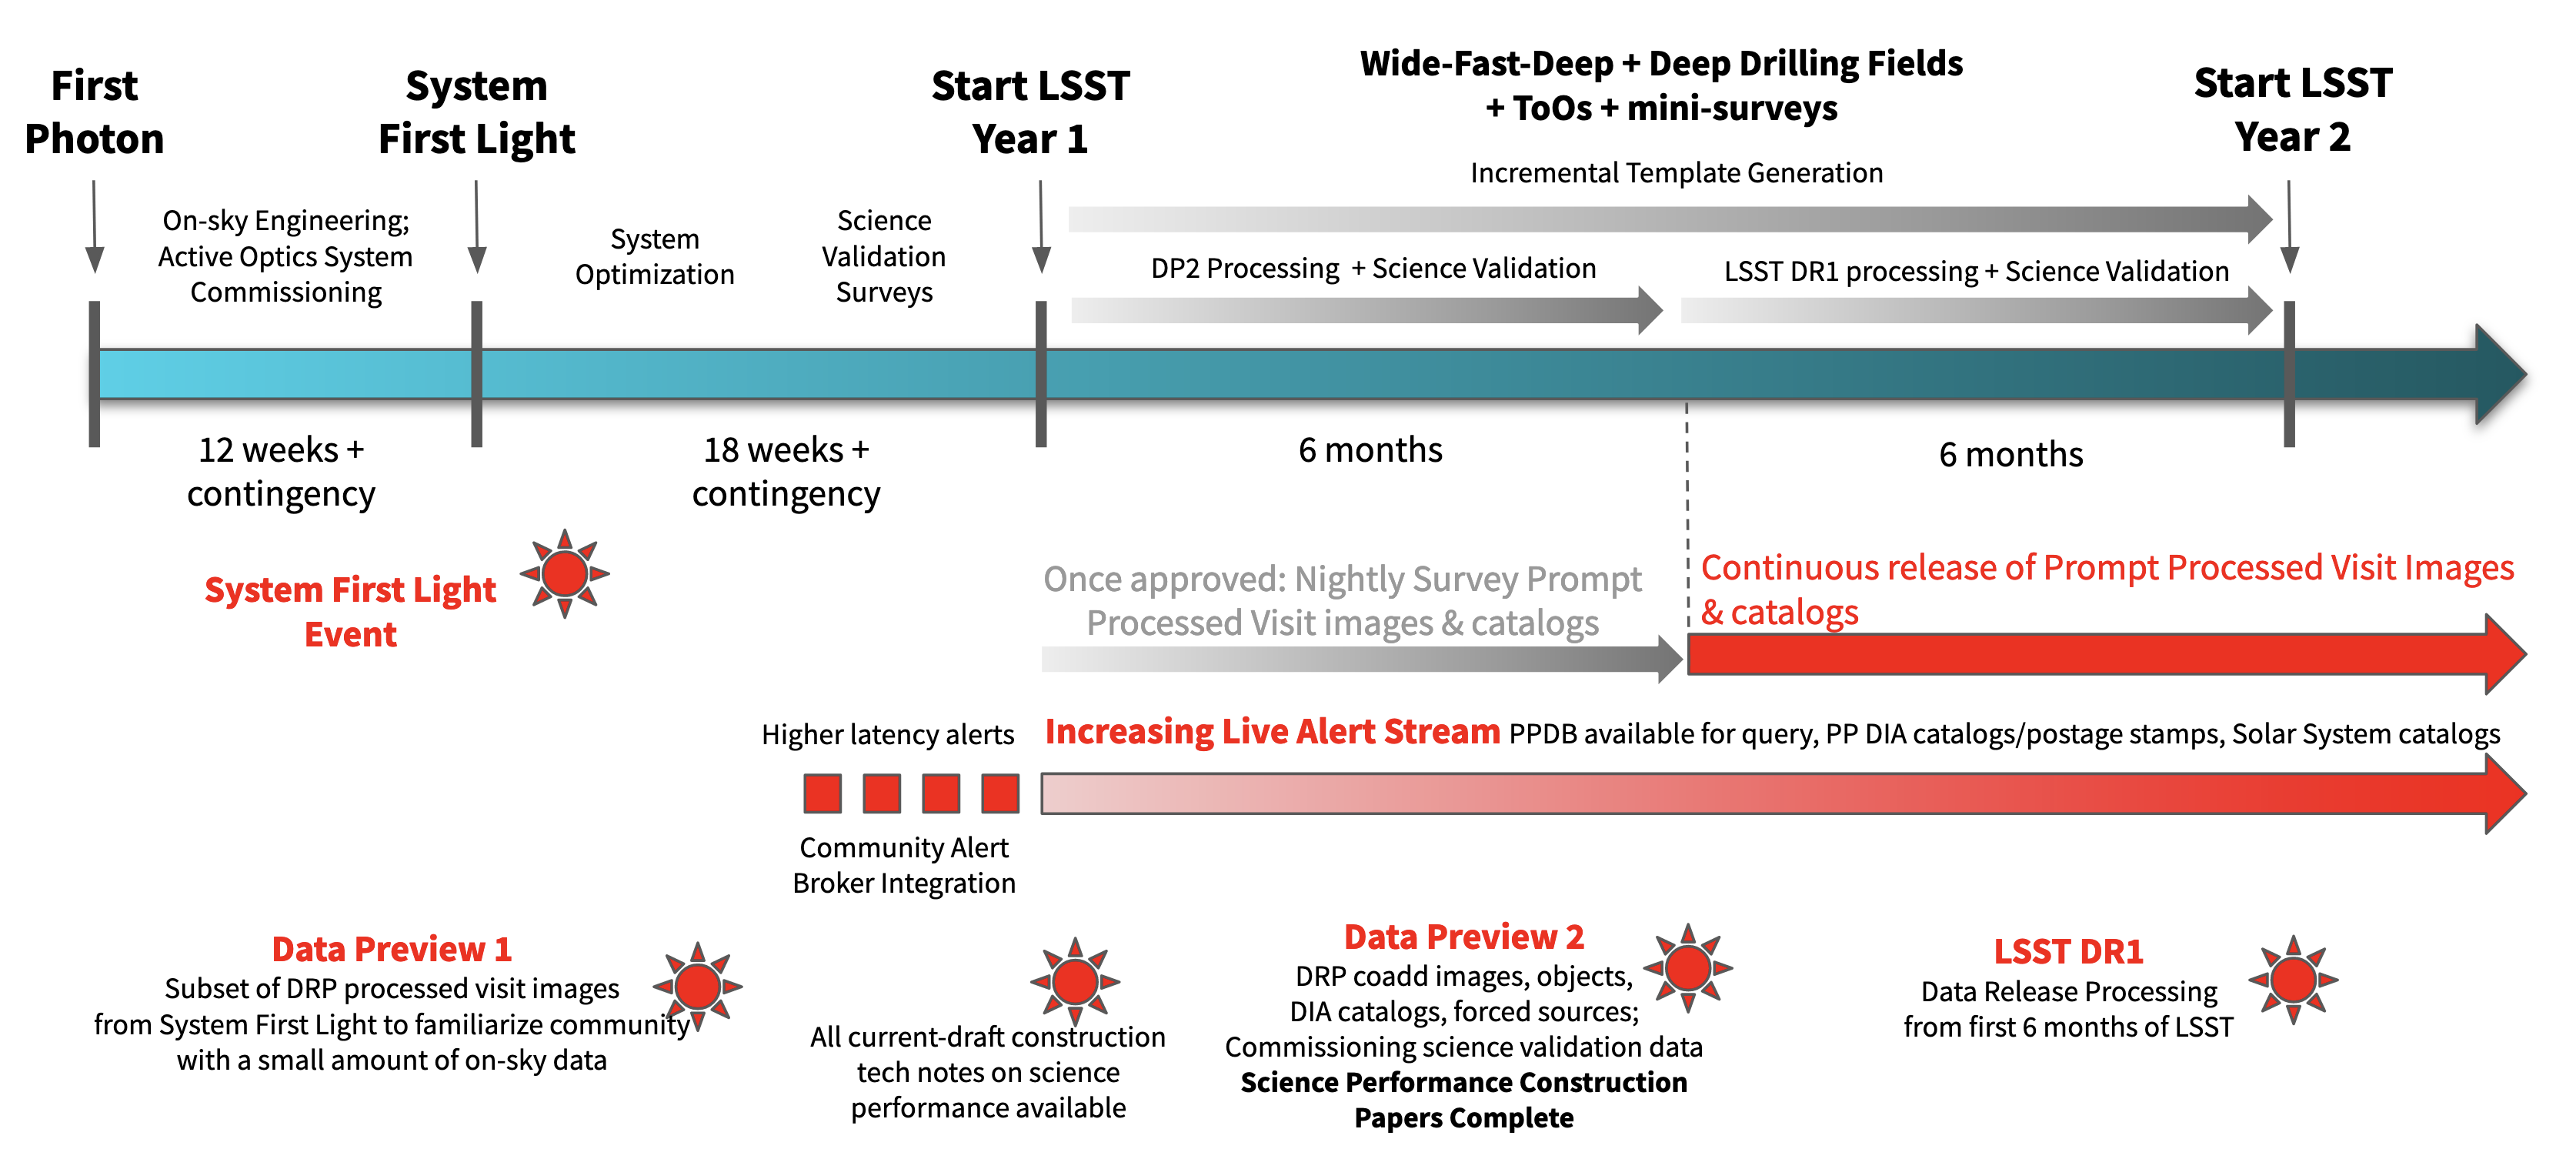
\includegraphics[width=1.0\textwidth]{timeline.png}
  \caption{Expected timeline for release of Early Science data products and supporting documentation for the technical and scientific performance of Rubin Observatory.}
  \label{timeline}
\end{figure}

Information regarding the technical and scientific performance of Rubin Observatory will be made available to the science community via technotes (Section \ref{technotes}) and a set of Construction papers (Section \ref{publications}).

\begin{warning}[Drafting in progress!]
  %The timeline for the release of PVIs, and release of associated source catalogs, is being reviewed by the Project Change Control Board.
  %Release of associated source catalogs with the PVIs is not yet in the baseline.
  %The proposed timeline for the release of PVIs and release of associated source catalogs are in the Project review process and may be revised
  %The proposed timeline for release of PVIs is in the Project review process and may be revised.
  This document is still being drafted.
  Release of associated source catalogs with the PVIs is not in the baseline.
  The proposed timeline for the release of PVIs and release of associated source catalogs are in the Project review process. After that, this document will be revised accordingly.
\end{warning}

%To support early science by the community,
Rubin Observatory seeks to maximize opportunities for early science with LSST data by the community.
At the start of the LSST 10-year survey, if the processing pipelines are sufficiently stable, nightly Processed Visit Images (PVIs) and accompanying source catalogs will be released on a best-effort basis.
%At the start of the LSST 10-year survey, if the processing pipelines are sufficiently stable, nightly Processed Visit Images (PVIs) will be released on a best-effort basis.
Release is subject to all embargo requirements, with caveats and preliminary calibration information.
%as determined by the Project and reviewed by [the SAC?, Ops Data Release Board?]
%These would be labeled as Preliminary Data, with
%There will be caveats and preliminary information about calibration.
% and no Project support for use until DP2.
%After the Data Preview 2 release
%Within 6 months following the start of LSST, PVIs will be released within the standard time window for steady-state LSST operations (see \citedsp{RTN-011}).
Within 6 months following the start of LSST, PVIs and source catalogs will be released within the standard time window for steady-state LSST operations (see \citedsp{RTN-011}).

\section{Commissioning Era Information Sharing Policies}
\label{policy}

\subsection{Summary}

%Project team members must follow policies for embargoed data products described in the Vera C. Rubin Observatory Data Policy \citedsp{RDO-013} and Project Publication Policy \citedsp{LPM-162}.
%, and Rubin Observatory Data Security Standards Implementation (DMTN-199).
All pixel images and representations of pixel images of any size field of view, including individual visit images, coadd images, and difference images based on LSSTCam commissioning on-sky observations are embargoed for a period of at least 30 days, with the exception of alert postage stamp images.

During the period from installation of LSSTCam on the telescope to the release of Data Preview 2, all communications (including informal discussion) regarding proprietary engineering and on-sky data with LSSTCam are internal to Rubin Project by default.
Outward-facing communications, including all on-sky LSSTCam images, are reviewed by SIT-Com leadership, the Rubin Celebrations Organizing Committee (RCOC) and its relevant subgroups, and the Communications team, and are approved for release by the Project Director or designated alternate.

Example outward-facing communications:

\begin{itemize}

  \item Weekly digests and News stories on \href{https://rubinobservatory.org/}{Rubin Observatory webpages}

  \item \href{https://www.lsst.org/about/project-status}{Published project status webpage}

  \item Rubin Observatory press releases / media events

  \item Released photographs, plots, and on-sky images

  \item Approved technotes (see Section \ref{technotes})

\end{itemize}

Free and unfettered communication among Project team members is essential for commissioning success.
%For proprietary data,
Project team members are required to use only approved Project tools, platforms, and processes for communication, data access and analysis, documentation, software development, work management, etc.
Derived data products are not subject to those restrictions, but are embargoed until approval for release (see Section \ref{technotes}).
In practice, we expect most work done by the Project team on the commissioning data to be done within protected directories at the Rubin US Data Facility at SLAC.

Prior to the release of associated data products as part of the Early Science program, derived data products from LSSTCam on-sky commissioning data may be shared beyond the Project team only in the following situations:

\begin{enumerate}

  \item the derived data product has been approved for release in one of the official Rubin Observatory outward-facing communication channels;

  \item the derived data product is documented as part of an approved technote (see Section \ref{technotes}).

\end{enumerate}

Derived data products that represent visit, coadd, and difference images from LSSTCam on-sky commissioning, with the exception of alert postage stamp images, are embargoed for a period of at least 30 days following the observation.
%not corresponding to artificial Earth-orbiting satellites

%Derived data products based on commissioning on-sky data will not be released for at least 80 hours following the observation.

During the on-sky commissioning period with LSSTCam, members of the Project team are allowed to discuss technical details of their work outside the team, and they may freely discuss aspects that do NOT relate to specific on-sky data products from LSSTCam or interim science performance.
Discussion on the general status of commissioning should refer to Project-approved resources for information on the progress of commissioning activities (e.g., digests, news stories, published Project status on the Rubin Observatory website).

\subsection{AuxTel, Electro-optical Datasets from ComCam and LSSTCam, and Non-proprietary Precursor Datasets}

Derived data products resulting from analysis of AuxTel datasets, and electro-optical datasets from ComCam and LSSTCam, as well as non-proprietary precursor datasets (e.g., HSC and DECam) and non-proprietary simulated datasets (e.g., DESC DC2) may be openly discussed and shared.

%\subsection{Transferring Data Products from Rubin Computing Facilities}

%In general, it is NOT permitted to copy/move data products from Rubin Observatory computing facilities to other locations without explicit permission.
%See Rubin Observatory Data Security Standards Implementation (DMTN-199).

\subsection{Technotes}
\label{technotes}

\href{https://developer.lsst.io/project-docs/technotes.html}{Technotes} are a way for Rubin Observatory team members to write standalone documents that are native to the web, can be cited in literature, and are easy to write, publish, and update.
A listing of technotes is available at \url{www.lsst.io}.

During the on-sky commissioning period with LSSTCam, technotes are anticipated to be one of the primary mechanisms to share information about Rubin Observatory data with the science community.
Project team members are encouraged to document their analyses in the form of technotes, e.g., to describe an algorithm or analysis software, to characterize and/or propose a solution to an outstanding issue, or to present the results of a science verification / validation study.
Technotes may present science validation analyses, but are not intended to include novel scientific results / discoveries.
Each technote should have a well defined scope.

Prior to the associated Early Science release, technotes that involve proprietary on-sky LSSTCam data must be first drafted in a restricted space and reviewed/approved by the Project using a standard checklist in a timely manner before posting.
This process will ensure that released technotes meet basic standards for documentation quality and conform to Rubin Observatory information release policies.
As living documents, technotes may describe work in progress and may be updated as studies progress.
Once released, updated technote versions must maintain compliance with the approval checklist criteria.

Derived data products may be documented and shared via technotes that have been approved for public release.

%\section{Frequently Asked Questions}

\subsection{Presentations}

When presenting on Rubin Observatory technical and scientific performance at institutional meetings, LSST Science Collaboration meetings, scientific conferences, seminars and colloquia, etc., Project team members are responsible for following presentation guidelines adopted by the Project.
The presentation content related to Rubin Observatory technical and scientific performance may only include released materials.
%Approved derived data products may be openly discussed.
%When presenting on Rubin Observatory at
%\href{https://www.lsst.org/scientists/codes-of-conduct}{professional standards of conduct} adopted by the Project.

\subsection{External Proposals}

Members of the Project team are welcome to include descriptions of their commissioning activities to support external grant proposals and observing proposals.
Embargoed information cannot be included, except with specific approval of the Rubin Observatory Project Office.
Approved derived data products may be included.

\subsection{Student Dissertations/Theses}

The commissioning-era information sharing policies apply to student dissertations and theses.
% will follow the same policies for information sharing.
Students on the Project team who intend to report results from analysis of unreleased on-sky LSSTCam commissioning data as part of their dissertation/thesis are advised to document their work via technotes so that approved results can be shared outside the Project team.
%, allowing time for approval prior to circulating their draft with others outside the Project team.
%consult with
%In order to support students on the Project team who plan to use proprietary on-sky commissioning data as part of their dissertation or thesis,
%the students and their academic advisors should consult with the SIT-Com leadership well in advance of circulating their draft to anyone outside the Project.
% to discuss the expected commissioning time.
%of their expected graduation.

\section{Peer-reviewed Journal Publications}
\label{publications}

The Project Publication Policy \citedsp{LPM-162} covers all publications that describe Project-funded work to design, develop, construct, commission, or operate the Observatory, and all publications based on access to non-public intellectual property of the Project or proprietary information related to the Project.

Rubin Observatory is drafting a set of \textbf{Construction Papers} to be published in peer-reviewed journals as part of the body of documentation to describe the technical and scientific performance of the as-built system.
The Construction Papers describe infrastructure work by Project team members and are thus covered by the Project Publication Policy.
Construction Papers that describe scientific performance will be completed by the Data Preview 2 release date in order to support the community to write science papers based on Early Science data products.

Members of the Project team might also contribute to science papers that use released commissioning data from the Early Science program.
The Rubin Data Policy \citedsp{RDO-013} states:

\begin{emph}
  {DPOL-516 Science Data from Commissioning: Scientific analysis of the commissioning data will be an integral and necessary part of the science verification process.
  All commissioning data used for science will be released to all LSST Users prior to any publication by anyone.
  Members of the Project team may not submit science papers to a journal and/or the arXiv based on commissioning data prior to the release of those data to LSST Users, but they may undergo the Rubin Observatory Publication Board process (this board is part of the construction project, not operations) in advance of the release of those data.}
\end{emph}

%, unless those papers have Project team co-authors and include previously unpublished aspects of Observatory science performance.
%In that scenario, the specific parts of the paper that
%also include previously unpublished aspects of Observatory science performance, which must be reviewed by the Project.

%Members of the Project team are free to collaborate with others beyond the Project team on science papers that use Early Science data.
%Science paper processes, including reviews and approvals, are in the purview of the LSST Science Collaborations.

Science papers that rely only on released Early Science data products are NOT covered by the Project Publication Policy.\footnote{Authors should consult with the Rubin Observatory Publication Manager if they are uncertain whether a manuscript in preparation would be classified as infrastructure work covered by the Project Publication Policy.}
%Science paper processes, including reviews and approvals, are in the purview of the LSST Science Collaborations.
However, for science papers that include members of the Project team as authors, we suggest the following guidelines to promote transparency:

%and that describe work that began prior to the release of the Early Science data products,
%For science papers that include members of the Project team as co-authors and that
%and that describe work on data not yet released, we suggest the following guidelines to promote transparency:

\begin{itemize}

  \item Project team members may begin writing science papers based on commissioning data prior to the release of associated Early Science data products.
  Those science papers may not be submitted until the associated data products are released.

  \item Project team members are free to collaborate with others beyond the Project team on science papers that use Early Science data.
  The Project team authors are welcome to inform their collaborators about their intent to write such science papers prior to the release, but no aspects of any science result may be shared until after the associated data release.

  \item The authors are encouraged, but not obliged, to announce plans for science publications as soon as possible within the Project team and welcome collaboration.
  They should discuss relevant publication policies (e.g., from LSST Science Collaborations) well in advance to avoid possible tensions.

  %\item Since members of the Project team are free to collaborate with others beyond the Project team on science papers that use Early Science data.
  %Prior to the release of the Early Science data products, the Project team authors are welcome to inform their collaborators beyond the Project team about their intent to write early science papers; transparency is encouraged.
  %However,

  %scientific results may NOT be shared outside the Project team prior to the associated data release.

  %beyond those directly related to technical and scientific performance

  %\item The authors are welcome to inform their collaborators beyond the Project team about their intent to write early science papers; transparency is encouraged.
  %However, prior to the public release of data, members of the Project team may not share outside the Project any aspect of any science result obtained with those data.
  %For example, Project team members may not share with their collaborators outside the project any information about specific science results until the data are public.
  %\item Members of the Project team are free to collaborate with others beyond the Project team on science papers that use Early Science data.
  %The authors are welcome to inform their collaborators beyond the Project team about their intent to write such science papers; transparency is encouraged.
  %Science paper processes, including reviews and approvals, are in the purview of the LSST Science Collaborations.

  \item A technote describing science validation analysis of on-sky commissioning data could become the basis for (parts of) a science paper submitted to a peer-review journal / the arXiv.
  %Technotes are intended to describe Rubin Observatory infrastructure and science validation work, including analyses of technical and scientific performance during commissioning.

  %\item Scientific results beyond those directly related to technical and scientific performance may NOT be shared outside the Project team prior to the associated data release.
  %While commissioning data products may NOT be shared prior to release, derived data products may be shared via approved technotes that can then be openly discussed.

  \item The authors are encouraged to circulate a draft within the Project team for comments several weeks in advance of submission / public posting.
  Since these non-infrastructure publications are not covered by the Project Publication Policy, there is no formal review by Rubin Observatory.

  \item The authors should encourage co-authorship as appropriate to recognize the contributions of other Project team members.
  No one should be listed as a co-author without their explicit permission.

  \item The publication should reference appropriate Construction Papers, technotes, and other Rubin Observatory documentation.

\end{itemize}

Under extraordinary circumstances, the Project may publicly release scientific results and associated data earlier than the timeline shown in Figure \ref{timeline}.

\section{Transition to Operations}
\label{operations}

The Operations team is working on methods and guidelines to enhance early science publicity.
The Project team will be encouraged to follow those guidelines and to help showcase the science results and potential of Rubin Observatory.

The evolution of the policies and guidelines described here into the Operations period is in the Operations team purview.


\appendix
% Include all the relevant bib files.
% https://lsst-texmf.lsst.io/lsstdoc.html#bibliographies
\section{References} \label{sec:bib}
\renewcommand{\refname}{} % Suppress default Bibliography section
\bibliography{local,lsst,lsst-dm,refs_ads,refs,books}

% Make sure lsst-texmf/bin/generateAcronyms.py is in your path
\section{Acronyms} \label{sec:acronyms}
\addtocounter{table}{-1}
\begin{longtable}{p{0.145\textwidth}p{0.8\textwidth}}\hline
\textbf{Acronym} & \textbf{Description}  \\\hline

ComCam & The commissioning camera is a single-raft, 9-CCD camera that will be installed in LSST during commissioning, before the final camera is ready. \\\hline
DC2 & Data Challenge 2 (DESC) \\\hline
DESC & Dark Energy Science Collaboration \\\hline
DMTN & DM Technical Note \\\hline
DOE & Department of Energy \\\hline
DR1 & Data Release 1 \\\hline
HSC & Hyper Suprime-Cam \\\hline
LPM & LSST Project Management (Document Handle) \\\hline
LSST & Legacy Survey of Space and Time (formerly Large Synoptic Survey Telescope) \\\hline
NSF & National Science Foundation \\\hline
RDO & Rubin Directors Office \\\hline
RTN & Rubin Technical Note \\\hline
SE & System Engineering \\\hline
SIT & System Integration, Test \\\hline
SLAC & SLAC National Accelerator Laboratory \\\hline
US & United States \\\hline
\end{longtable}

% If you want glossary uncomment below -- comment out the two lines above
%\printglossaries





\end{document}
